\section{USER}
    \subsection{Home}
        \begin{figure}[H] \noindent \centering
            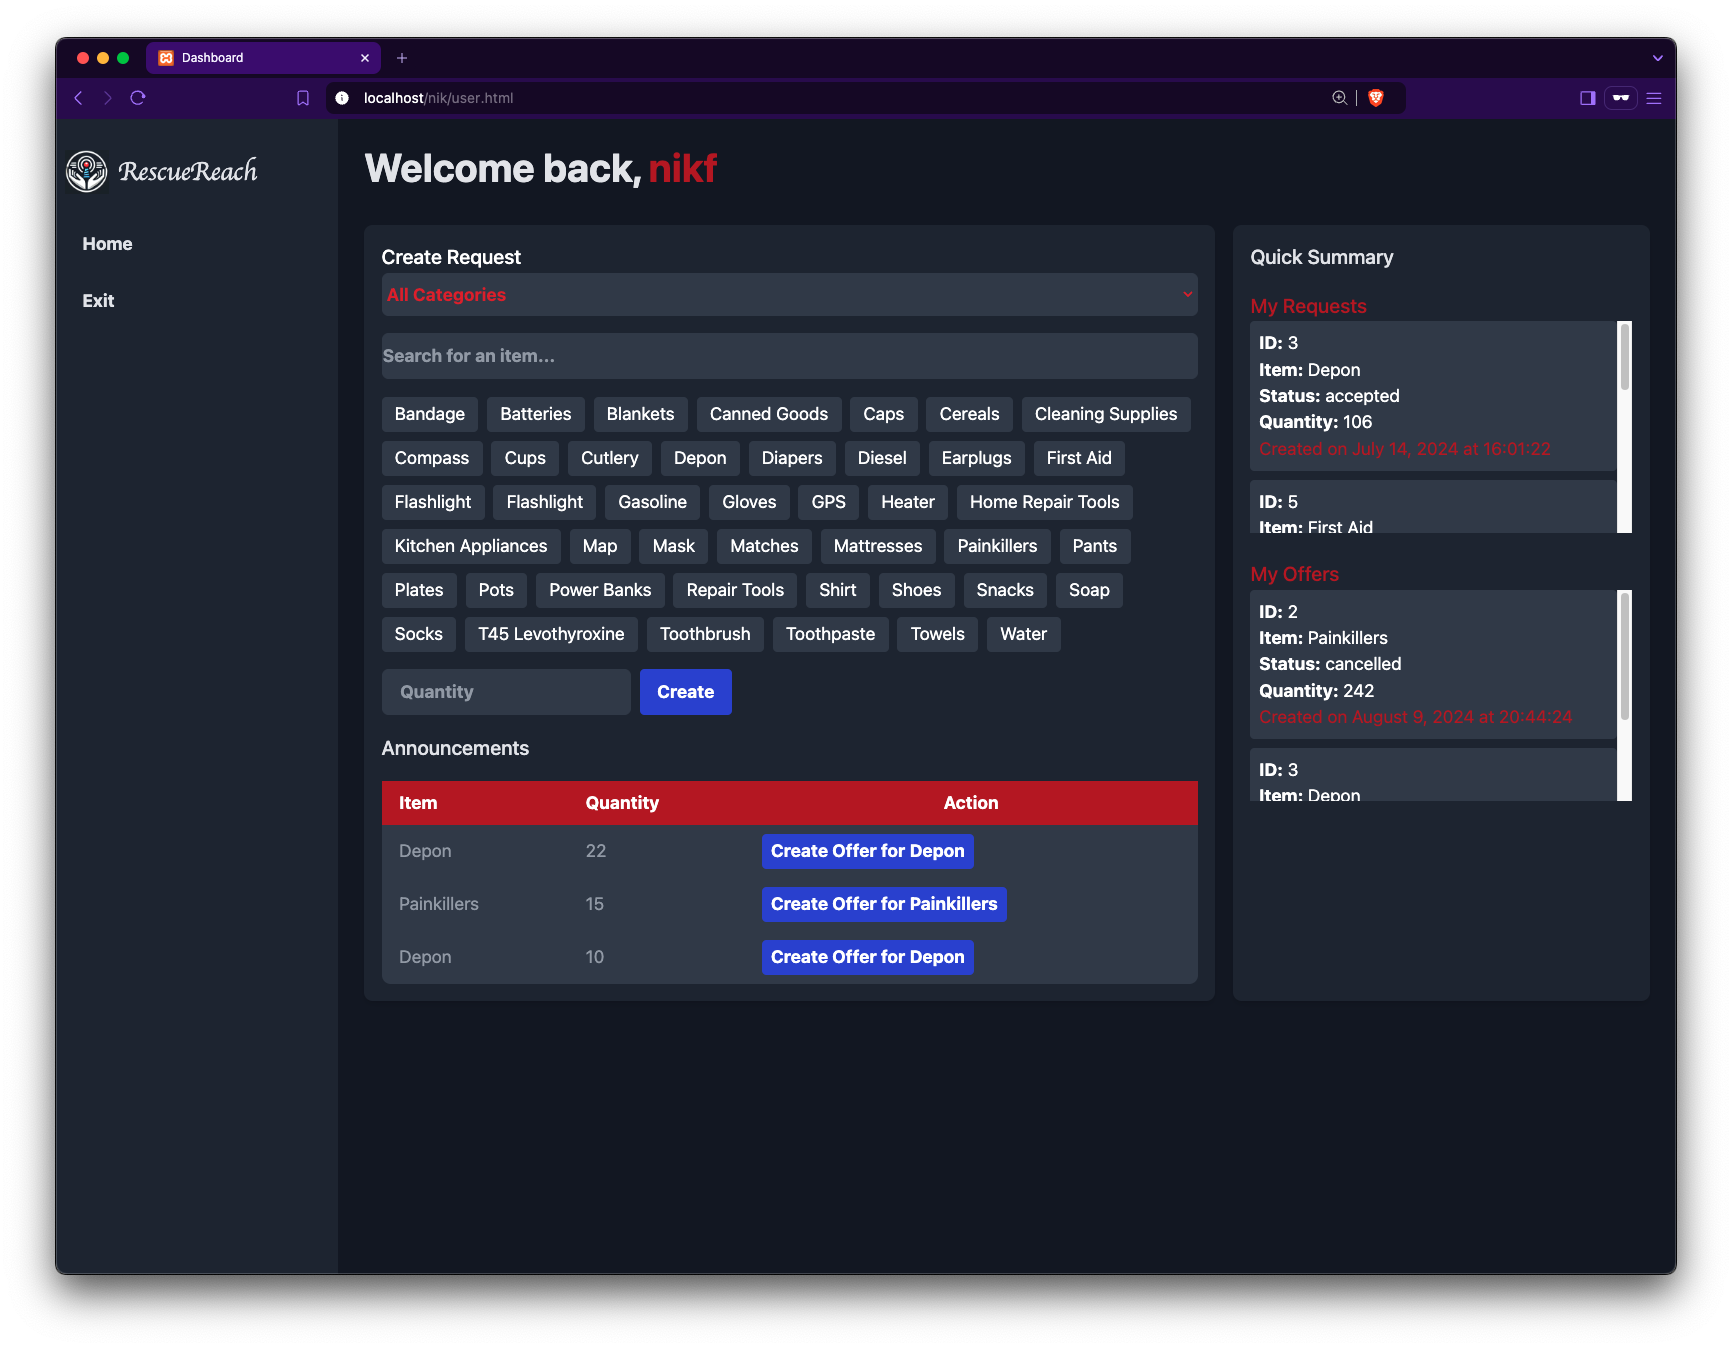
\includegraphics[width=0.9\textwidth]{img/user-dashboard}
            \caption{Αρχική σελίδα πολίτη}
        \end{figure}

    Πατώντας πάνω στο username, εμφανίζεται μια φόρμα όπου ο χρήστης μπορεί να αλλάξει τα στοιχεία του.
    Τα στοιχεία του φορτώνονται μέσω της \verb|get_user_data.php| και \verb|update_user.php|.

    Οι users μπορούν να δουν όλα τα αντικείμενα της βάσης, και να κάνουν request για κάποιο.
    Επίσης μπορούν να δουν τις ανακοινώσεις της βάσης και να κάνουν κάποιο offer.
    Οι πληροφορίες γίνονται fetch μέσω της \c{fetchTasks()}, \c{loadCategoriesAndItems()} και \c{loadAnnouncements()},
        και εμφανίζονται μέσω της \c{displayItems()}.
    Για να γίνουν τα requests, στέλνεται AJAX request στη \c{insert\_requests.php}, ενώ για τα offers στέλνεται AJAX request
        στη \c{create\_offers.php} με τα κατάλληλα Event Listener που αντιστοιχούν στα κουμπιά που δημιουργούνται.

    Στα δεξιά μπορούν επίσης να δουν τα requests και τα offers που έχουν κάνει, τα οποία γίνονται populate μέσω της \c{fetchTasks()}.

    \begin{figure}[H] \noindent \centering
        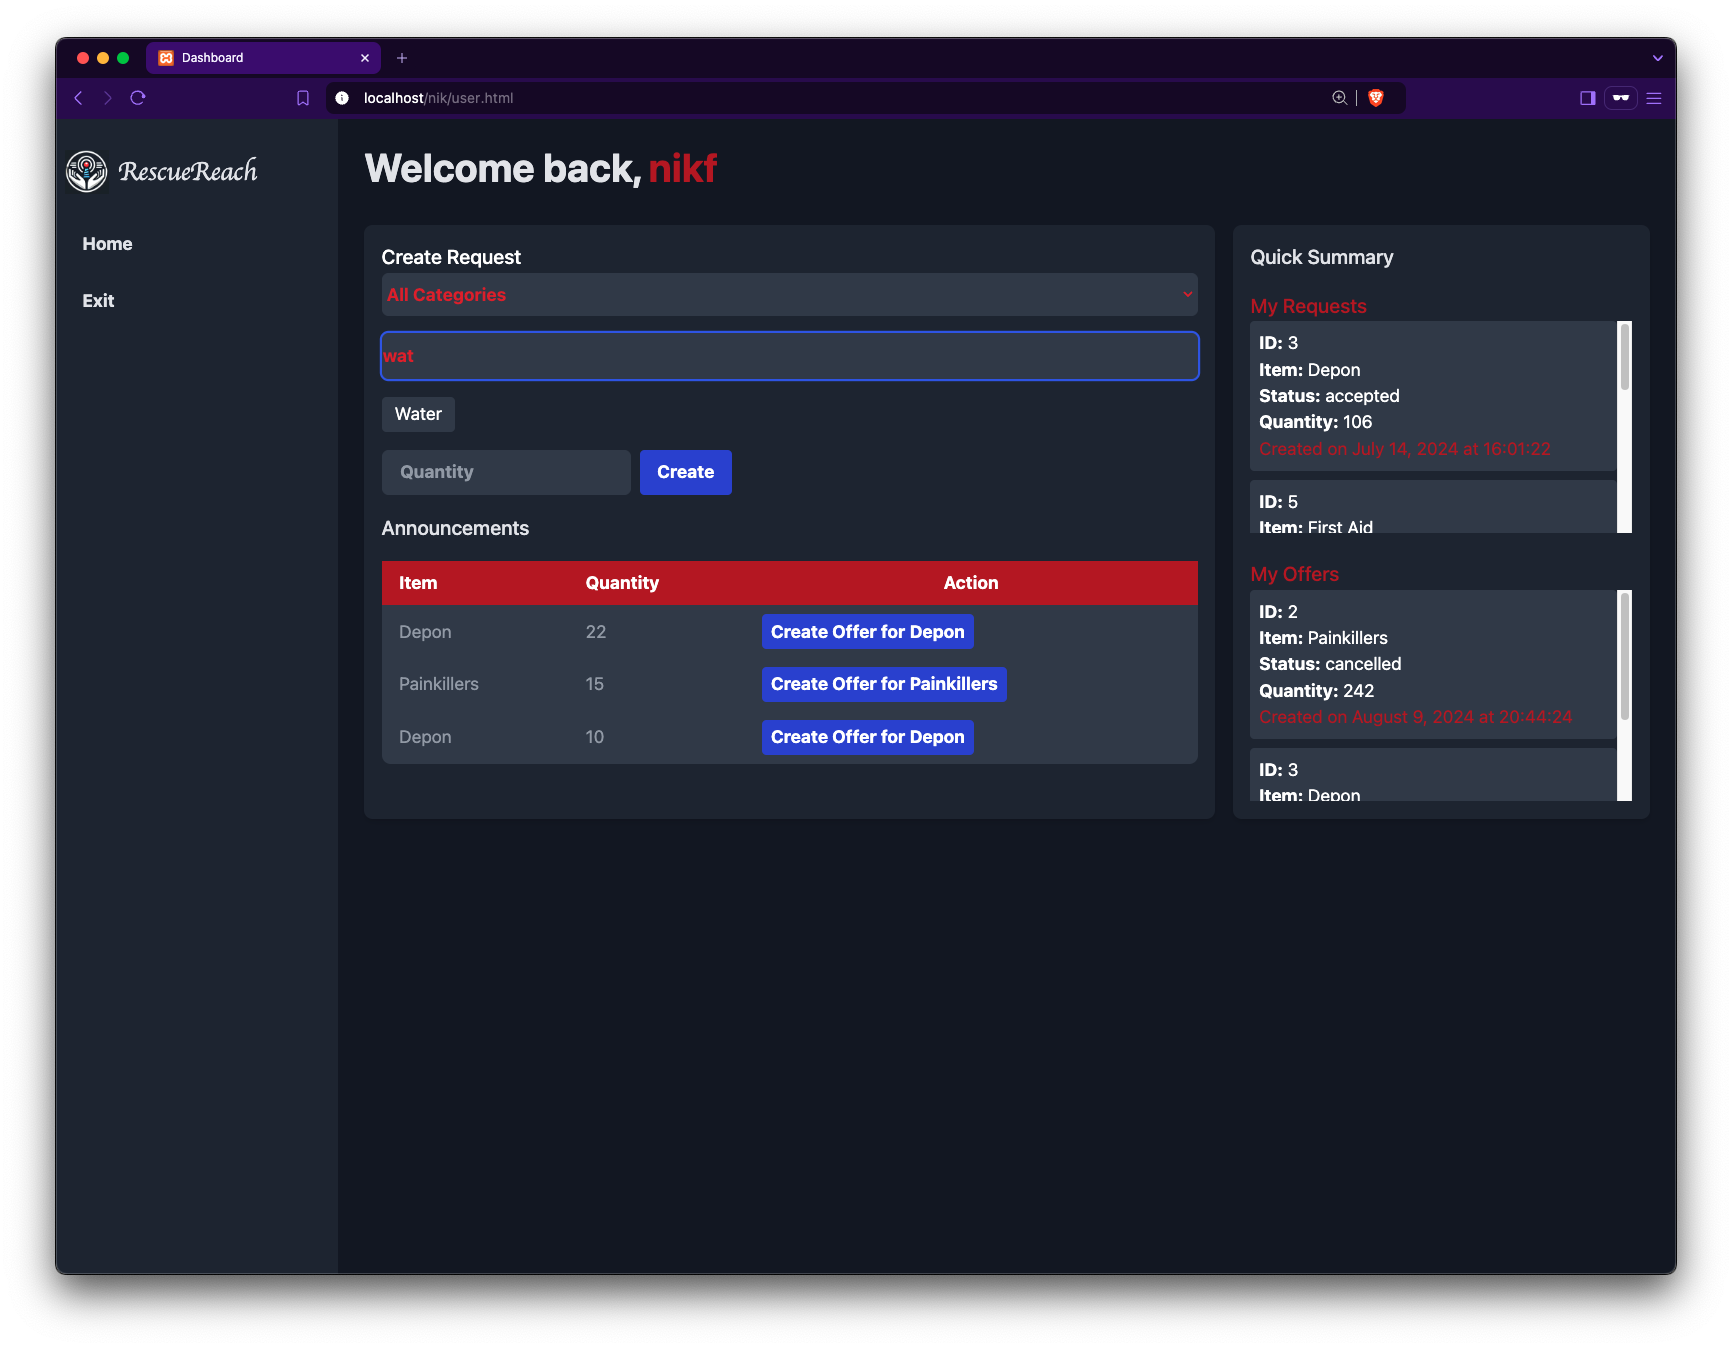
\includegraphics[width=0.8\textwidth]{img/user-dashboard_2}
        \caption{Αναζήτηση για συγκεκριμένο προϊόν.}
    \end{figure}